Word-level analysis is the first phase of the event detection algorithm, focused on obtaining a set of candidate words for event representation. We do not yet perform the actual event detection, which are addressed in the next chapter, but merely extract a subset of words carrying enough information to be considered representative.

Here we work with the assumption that an event can be detected by observing the frequencies of individual words over time and grouping together those words which appear in similar documents during similar time periods \citep{event-detection, parameter-free}. This corresponds to an event being often mentioned in the text stream around the period when it actually occurred. Of course, not all words are representative of an event, so we will have to impose a criterion of a ``word eventness''.

\cite{event-detection} also distinguished between periodic and aperiodic words, where periodic words are mentioned with a certain period (these words are related for example to sport matches played every weekend, weather forecasts reported every day, etc.) Consequently, the authors divided the words into two groups by their periodicity, and detected events from each group separately. However, during our evaluation, some word periodicities were misclassified. This would cause an event represented by those words to be split into a ``periodic part'' and an ``aperiodic part''. Therefore, we detect events from all ``eventful'' words at once, and examine the periodicities of the events later on.

\begin{figure}
\centering
\begin{subfigure}{.5\textwidth}
  \centering
  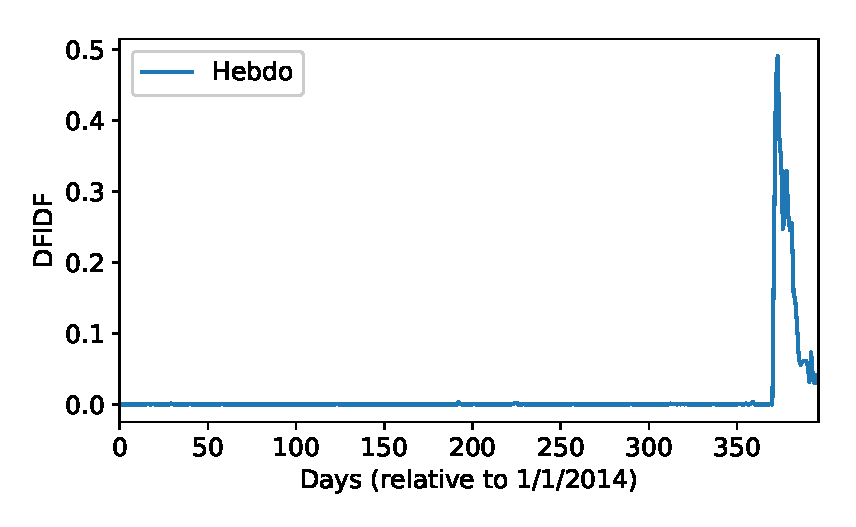
\includegraphics[width=\linewidth]{21255}  % Hebdo
  \caption{Aperiodic word}
  \label{fig:hebdo}
\end{subfigure}%
\begin{subfigure}{.5\textwidth}
  \centering
  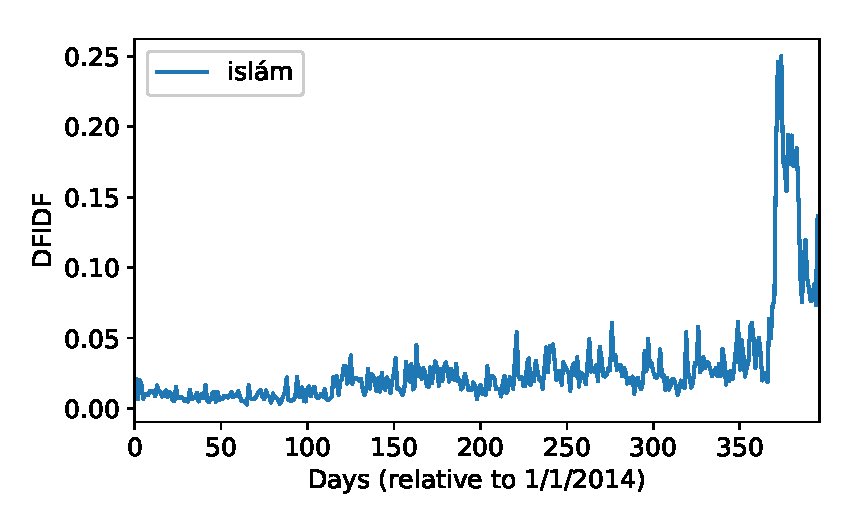
\includegraphics[width=\linewidth]{84055}  % islam
  \caption{Aperiodic word misclassified as periodic}
  \label{fig:islam}
\end{subfigure}
\caption{Trajectories of the words \textit{Hebdo} and \textit{Islam}, respectively. Both of these words are related to the shooting in Charlie Hebdo offices in Paris on January 7, 2015. However, the original method classifies the word \textit{Islam} as periodic with period of 198 days. If we detected events separately from periodic and aperiodic words, the event ``Charlie Hebdo attack'' would be split into at least two, causing redundancy.}
\end{figure}


At first, we construct a trajectory of each word --- a measure of word frequency over time. Then, we apply signal processing techniques which will be used to determine the eventness of each word. The same techniques will be later used to determine the event periodicities in \autoref{chap:document-retrieval}. Once we have a notion of word eventness, we extract a small subset of words to be considered for further analysis, and discard the rest.

These word trajectories will then be examined for so called ``bursts'' in frequency, where a word would suddenly start appearing in a large number of documents during a short time period. Should a number of words appear in similar documents with overlapping bursts, it may be an indicator that an event worthy of attention occurred.

One thing to note is that the frequency of a word is, by itself, not a good indicator of a word importance.
Stopwords appearing in most documents, such as conjunctions, prepositions, etc. do not carry any information and should be ignored. Therefore, we utilize the parts of speech tagging performed earlier and limit our analysis to Nouns, Verbs, Adjectives and Adverbs only. This limits the number of stopwords appearing in the stream, though some remain. These will need to be filtered by other means, as we will see in this chapter.

\begin{figure}
\centering
\begin{subfigure}{.5\textwidth}
  \centering
  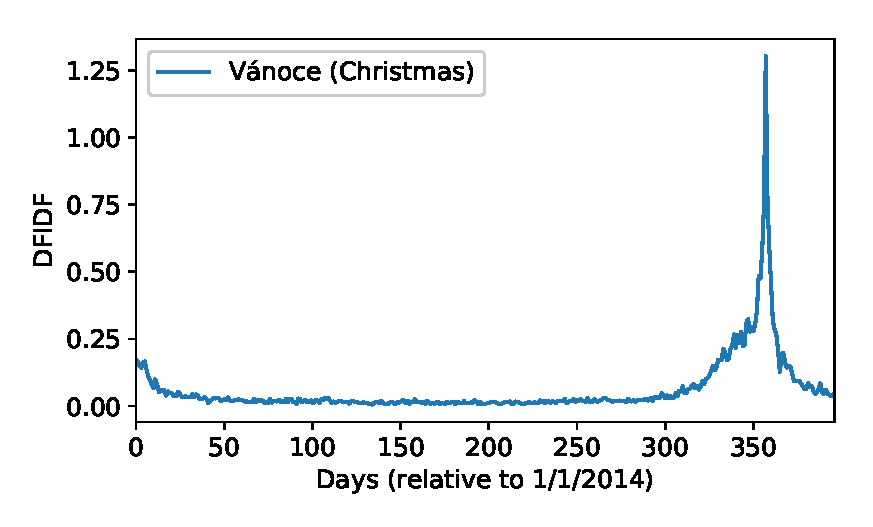
\includegraphics[width=\linewidth]{60141}  % Vanoce
  \caption{Eventful word}
  \label{fig:vanoce}
\end{subfigure}%
\begin{subfigure}{.5\textwidth}
  \centering
  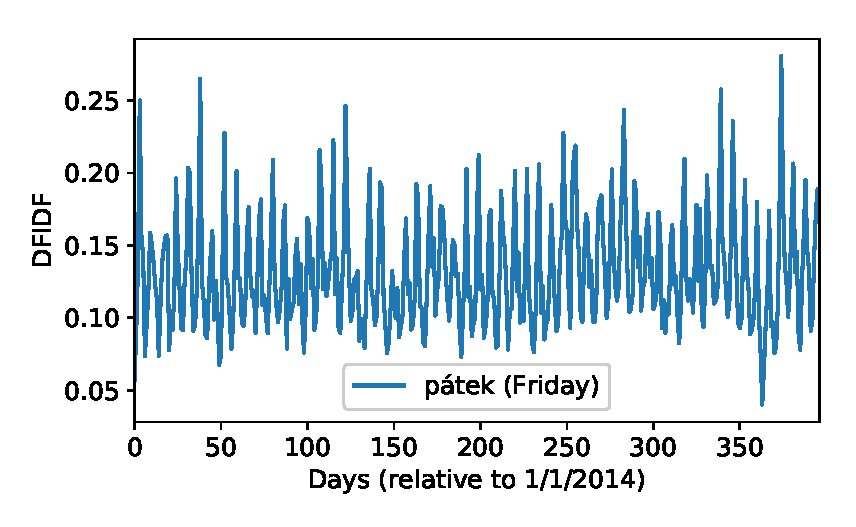
\includegraphics[width=\linewidth]{116963}  % patek
  \caption{Stopword}
  \label{fig:patek}
\end{subfigure}
\caption{(a) Trajectory of an eventful word \textit{Christmas}. (b) Trajectory of a stopword \textit{Friday} with period of 7 days.}
\end{figure}

We ignore the documents and focus entirely on word analysis up until \autoref{chap:document-retrieval}. There, we use the words assembled into events to query the document collection, obtaining the event-related documents. The core of this algorithm is taken from \cite{event-detection}.


\section{Binary bag of words model}
To construct the word trajectories, we first need to know which words appear in which documents, as we are interested in the document frequency of each word. We create a binary bag of words model, which is represented by a binary matrix denoting the incidence of documents and words. This model completely ignores word order, which is neglected in this analysis.

It might seem that using only a simple \textit{binary} model, as opposed to one denoting, say, the frequency of words within the documents, results in a loss of information. While true, this model is not the target word representation --- we only need to know the word-document incidence to construct the word trajectories, which are then the desired output.

We define a term-document matrix $\bowmat \in \left\{ 0, 1 \right\}^{\doccount \times \featcount}$, where $\doccount$ is the number of documents and $\featcount$ is the total vocabulary size. The document collection can then be interpreted as a set of $\doccount$ observations, each consisting of $\featcount$ binary features. The matrix $\bowmat$ is defined as

\begin{equation} \label{eq:bow-matrix}
	\bowmat_{ij} =
	\begin{cases}
		1, & \text{document}~i~\text{contains the word}~j \text{;} \\
		0, & \text{otherwise.}
	\end{cases}
\end{equation}

Because every document contains only a small fraction of the vocabulary, the matrix $\bowmat$ consists mostly of zeroes. This allows us to store the matrix in a sparse format, which makes it possible to fit the matrix in memory. We use a sparse matrix instead of a more traditional inverted index \citep{information-retrieval}, because this representation allows us to vectorize some further operations.


\section{Computing word trajectories}
\cite{event-detection} defined the time trajectory of a word $w$ as a vector\\ $\vect{\traj}_{w} = \left[ \traj_{w}(1), \traj_{w}(2), \dots, \traj_{w}(\streamlen) \right]$ with each element $\traj_{w}(t)$ being the relative frequency of $w$ at time $t$ $(1 \leq t \leq \streamlen,\ 1 \leq w \leq \featcount)$. This frequency is defined using the DFIDF (Document Frequency-Inverse Document Frequency) score:

\begin{equation}
	\traj_{w}(t) = \underbrace{\frac{\text{\df}_{w}(t)}{\text{\doccount}(t)}}_{\text{DF}} \cdot \underbrace{\log{\frac{\doccount}{\text{\df}_{w}}}}_{\text{IDF}},
\end{equation}

where $\text{\df}_{w}(t)$ is the number of documents published on day $t$ containing the word $w$ (time-local document frequency), $\text{\doccount}(t)$ is the number of documents published on day $t$, $\doccount$ is the total number of documents and $\text{\df}_{w}$ is the number of documents containing the word $w$ (global document frequency).

The DFIDF score, defined by \cite{event-detection}, is a modification of the commonly used TFIDF (Term Frequency-Inverse Document Frequency) score \citep{tfidf, information-retrieval}, which measures the importance of a word within a document collection. The purpose of this modification is to include temporal information and measure the word importance over time.

To be able to compute these word trajectories efficiently using the matrix $\bowmat$, we define a utility matrix $\dtdmat \in \left\{ 0, 1 \right\}^{\doccount \times \streamlen}$ mapping the documents to their publication days:

\begin{equation}
	\dtdmat_{ij} =
	\begin{cases}
		1, & \text{document}~i~\text{was published on day}~j \text{;} \\
		0, & \text{otherwise}.
	\end{cases}
\end{equation}

Next, we sum the rows of $\bowmat$ together to obtain $\vect{\df} = \left[ \text{\df}_{1}, \text{\df}_{2}, \dots, \text{\df}_{\featcount} \right]$, and similarly the rows of $\dtdmat$ to obtain $\vect{\doccount}_{t} = \left[ \text{\doccount}(1), \text{\doccount}(2), \dots, \text{\doccount}(\streamlen) \right]$.

Finally, we compute the word trajectory matrix $\trajmat \in \R^{\featcount \times \streamlen}$, with trajectory of a word $w$, $\vect{\traj}_w \in \R^{\streamlen}$, being the $w$-th row of $\trajmat$.

The matrix $\trajmat$ is computed as follows:

\begin{equation}
	\trajmat =
		\underbrace{\text{diag} \left( \log{\frac{\doccount}{\vect{\df}}} \right)}_{\text{IDF}}
		\cdot
		\underbrace{\bowmat^{\T}
		\cdot \dtdmat
		\cdot \text{diag} \left( \frac{1}{\vect{\doccount}_{t}} \right)}_{\text{DF}}
\end{equation}

Now, having trained the Word2Vec model in \autoref{chap:data-preprocessing} and constructed the word trajectories, we obtained temporal and semantic representation of the words. Every word $w$ is represented by two vectors: $\embed_{w} \in \R^{100}$ being its Word2Vec embedding, and $\vect{\traj}_{w} \in \R^{\streamlen}$ its time trajectory. The trajectories will be further analyzed in this chapter, while both trajectories and Word2Vec embeddings will be used in \autoref{chap:event-detection} to group words into events.


\section{Spectral analysis}
Having constructed the word trajectories, we still need to decide which words are eventful enough. \cite{event-detection} interpreted the word trajectories as time signals, which allowed them to analyze the trajectories using signal processing techniques. They performed the analysis both to decide word eventness and to discover the word periodicity.

Unlike the original paper, we only analyze the signal power to decide which words are eventful enough. We will detect events from both periodic and aperiodic words at once, and decide the periodicity of the whole events in \autoref{chap:document-retrieval}.

We apply the discrete Fourier transform to the trajectories to represent each time series as a linear combination of $\streamlen$ complex sinusoids. We obtain $\mathcal{F} \vect{\traj}_{w} = \left[ X_{1}, X_{2}, \dots, X_{\streamlen}\right ]$ such that

\begin{equation}
	X_{k} = \sum_{t = 1}^{\streamlen}{\traj_{w}(t) \exp \Big(- \frac{2 \pi \mi}{\streamlen} (k - 1) t} \Big), ~ k = 1, 2, \dots, \streamlen.
\end{equation}

The measure of ``eventness'' of a word is simply its signal power. That can be determined from the power spectrum of each signal, estimated using the periodogram $\vect{P} = \left[ \|X_{1}\|^{2}, \|X_{2}\|^{2}, \dots, \|X_{\ceil{\streamlen / 2}}\|^{2} \right]$.

To measure the overall signal power, we define the dominant power spectrum of the word $w$ as the value of the highest peak in the periodogram, that is

\begin{equation}
	\text{DPS}_{w} = \max\limits_{k \leq \ceil{\streamlen / 2}}{\|X_{k}\|^{2}}.
\end{equation}


\begin{figure}[H]
\centering
\begin{subfigure}{.5\textwidth}
  \centering
  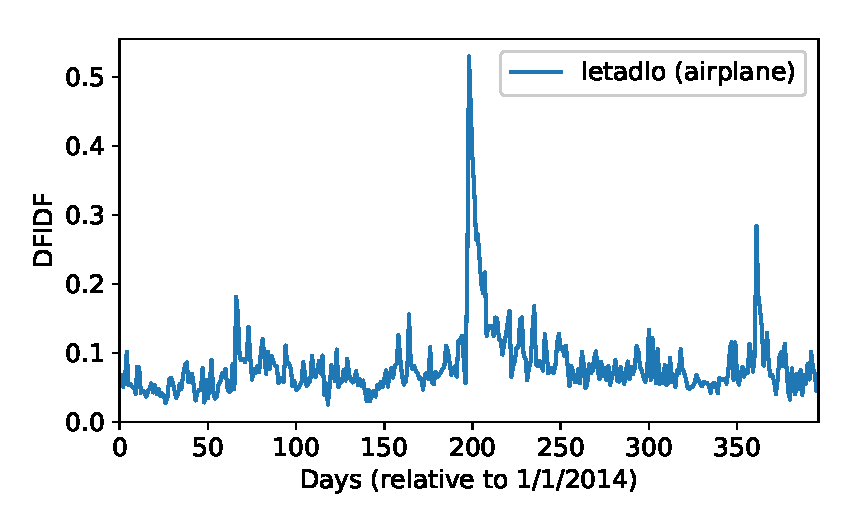
\includegraphics[width=\linewidth]{91143}  % letadlo
  \caption{Trajectory}
  \label{fig:letadlo}
\end{subfigure}%
\begin{subfigure}{.5\textwidth}
  \centering
  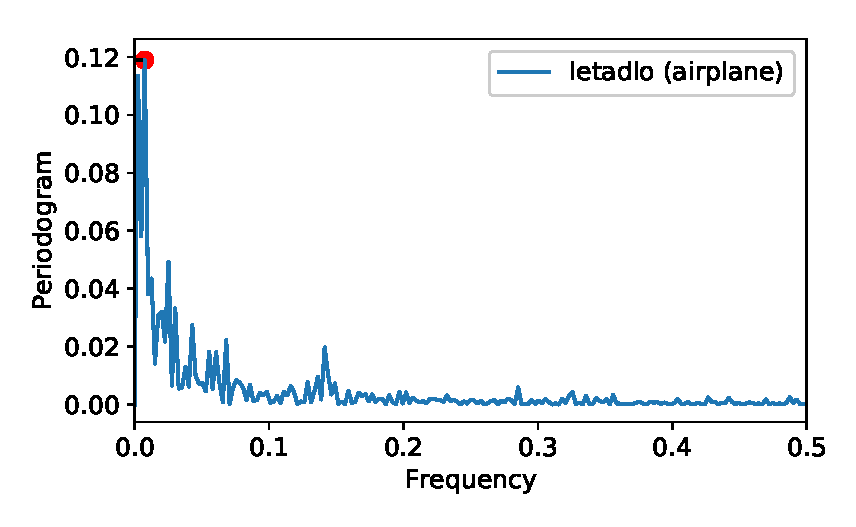
\includegraphics[width=\linewidth]{91143_periodogram}  % letadlo periodogram
  \caption{Periodogram with indicated DPS}
  \label{fig:letadlo-periodogram}
\end{subfigure}
\caption{Trajectory and periodogram of the word \textit{airplane}.}
\end{figure}

Finally, \cite{event-detection} define the set of all eventful words (EW) as those words whose trajectory signal is powerful enough. This corresponds to their occurrence in a large number of documents in a noiseless pattern:

\begin{equation}
	\text{EW} = \left\{ w \mid \text{DPS}_{w} > \textit{DPS-bound} \right\}.
\end{equation}

where \textit{DPS-bound} can be estimated using the \textit{Heuristic stopword detection} algorithm described in \cite{event-detection}. The algorithm computes the average trajectory value and DPS values from a given seed stopwords set. The DPS boundary is then defined as the maximum DPS value of the stopwords set.